\chapter{Návrh riešenia}
\section[Klasifikácia]{Klasifikácia na základe lokálnej informácie}

\subsection{Úloha klasifikátora}

V našej práci sme klasifikátor použili na zakomponovaní dodatočných informácií o sekvenciách do modelu zarovnania sekvencií. Dodatočné informácie sú poskytnuté formou anotácií k príslušným bázam.

V našich modeloch sme použili 2 typy klasifikátorov -- \textit{Match klasifikátor} a \textit{InDel klasifikátor}. Match klasifikátor sa klasifikátor určuje s akou pravdepodobnosťou sa majú dané dve pozície v sekvenciách zarovnať k sebe. InDel klasifikátor urcuje s akou pravdepodobnosťou má byť pozícia v príslušnej sekvencii zarovnaná s medzerou. Tieto pravdepodobnosti sú mierou istoty daného klasifikátora, a keďže tieto 2 klasifikátory sú nezávislé, súčet ich výstupov nemusí byť jedna.

\subsection{Random Forest}

\subsection{Match klasifikátor}

Match klasifikátor určuje, či sa dané dve pozície majú zarovnať k sebe. Jeho výstupom je číslo z intervalu $\left<0,1\right>$, pričom čím bližšie je toto čislo k 1, tým si je klasifikátor istejší, že dané 2 pozície sa majú zarovnať k sebe. Naopak, čím bližšie je k 0, tým si je viac istý, že by tieto pozície k sebe byť nemajú.

\subsubsection{Vstupné dáta}

Ako vstupné dáta dostane tento klasifikátor okolie okolo daných pozícií. Toto okolie budeme volať \textit{okno}.

Majme dve sekvencie, $X = x_1 x_2 \dots x_n$ a $Y = y_1 y_2 \dots y_n$ a pozície $i$ a $j$. Okno veľkosti $w$ obsahuje $x_{i - w/2}\dots x_i \dots x_{i + (1 + w)/2}$, $y_{j - w/2}\dots y_j \dots y_{j + (1 + w)/2}$ a všetky anotácie príslušných báz. (Obr. \ref{fig:window-m})

% \begin{figure}[htp]
%     \centering
%     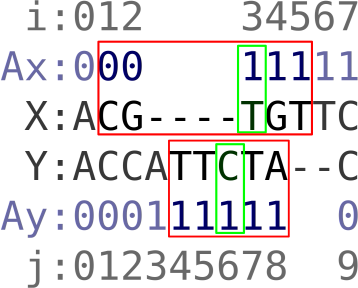
\includegraphics[width=.25\textwidth]{images/window_m}
%     \caption{Okno Match klasifikátora pre $i = 3$ a $j = 6$}
%     \label{fig:window-m}
% \end{figure}

\subsubsection{Trénovanie}
\todo

\subsection{InDel klasifikátor}

InDel klasifikátor určuje, či sa daná pozícia má zarovnať k medzere. Jeho výstupom je opäť  číslo z intervalu $\left<0,1\right>$, pričom čím bližšie je toto čislo k 1, tým si je klasifikátor istejší, že daná pozícia sa má zarovnať k medzere a čím bližšie je k 0, tým si je viac istý, že sa táto pozícia nemá zarovnať k medzere.

\subsubsection{Vstupné dáta}
Aj pri tomto klasifikátore použivame dve pozície prvá je pozícia v inzert sekvencii a ukazuje na bázu, na ktorú sa pýtame a druhá pozícia je v druhej sekvencii a ukazuje na medzeru - teda medzi dve bázy.

Majme dve sekvencie, $X = x_1 x_2 \dots x_n$ a $Y = y_1 y_2 \dots y_n$ a pozície $i$ a $j$. Nech $X$ je inzert sekvencie, potom okno veľkosti $w$ obsahuje $x_{i - w/2}\dots x_i \dots x_{i + (1 + w)/2}$, $y_{j - w/2}\dots y_j \dots y_{j + (1 + w)/2 - 1}$ a všetky anotácie príslušných báz. (Obr. \ref{fig:window-i})

% \begin{figure}[htp]
%     \centering
%     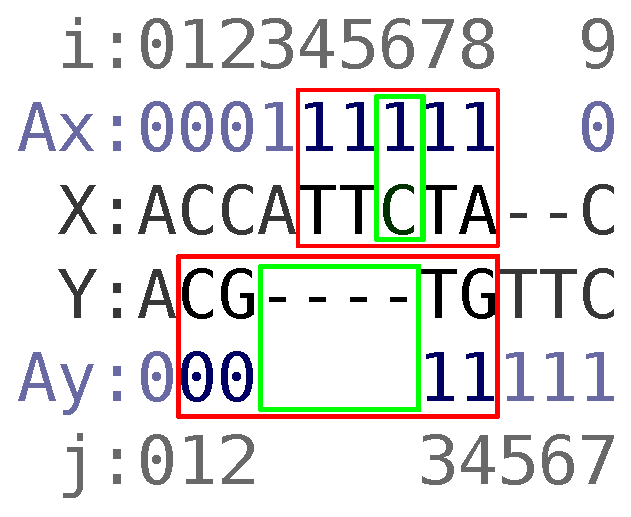
\includegraphics[width=.25\textwidth]{images/window_i}
%     \caption{Okno InDel klasifikátora pre $i = 3$ a $j = 6$}
%     \label{fig:window-i}
% \end{figure}

\begin{figure}[hp]
        \centering
        \begin{subfigure}[b]{0.35\textwidth}
                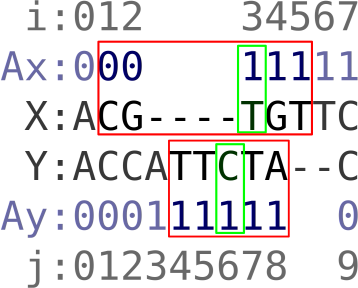
\includegraphics[width=\textwidth]{images/window_m}
                \caption{Match klasifikátor}
                \label{fig:window-m}
        \end{subfigure}%
        \qquad\qquad %add desired spacing between images, e. g. ~, \quad, \qquad etc.
          %(or a blank line to force the subfigure onto a new line)
        \begin{subfigure}[b]{0.35\textwidth}
                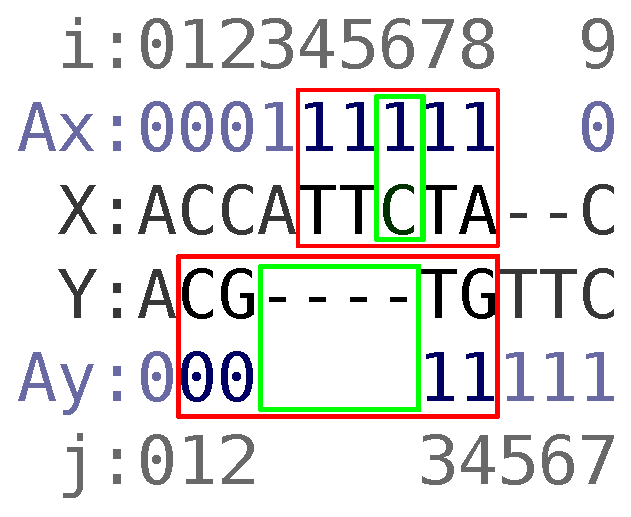
\includegraphics[width=\textwidth]{images/window_i}
                \caption{InDel klasifikátor}
                \label{fig:window-i}
        \end{subfigure}
        \caption{Okno klasifikátora pre pozície $i = 3$ a $j = 6$}
\end{figure}
\vspace{-1cm}

\subsubsection{Trénovanie}
\todo

\section{Modely}

V sekcii \ref{sec:hmm-alignment} sme si zadefinovali HMM pre zarovnávanie sekvenci (obr. \ref{fig:simple-model}).
V našom riešení sme predstavili 2 modifikácie pôvodného HMM na zakomponovanie dodatočnej informácie, pričom sme využili klasifikátory. V oboch modeloch sú klasifikátory rovnaké, aj s rovnakým postupom trénovania. Líši sa len trénovanie samotného HMM a architektúra modelu.

\subsection{Model s klasifikátorom ako emisiou}

V tomto modeli sme nahradili emisné tabuľky stavov výstupom z klasifikátora.
Model teda bude vyzerať rovnako, aj pravdepodobnosti prechodov zostanú, ale emisná pravdepodobnosť sa nahradí výstupom z klasifikátora.

\begin{figure}[htp]
    \centering
    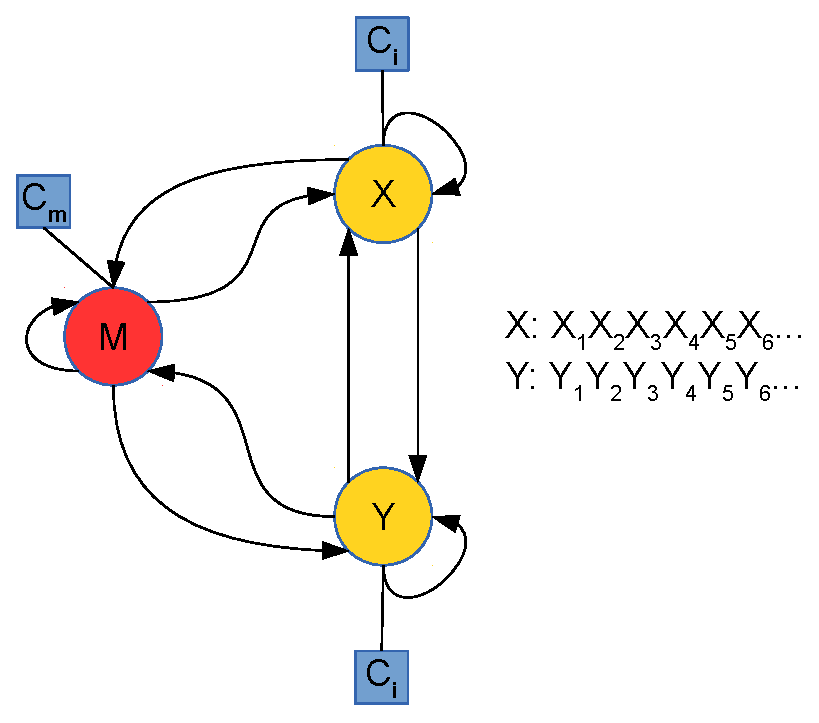
\includegraphics[width=.5\textwidth]{images/model_clf}
    \caption{Model s klasifikátorom ako emisiou}
\end{figure}


Problémom tohto modelu je, že výstup klasifikátora nezodpovedá emisným pravdepodobonstiam, ale akejsi istote klasifikátora o tom, že dve pozície majú byť zarovnané k sebe. Hodnoty z klasifikátora teda nesumujú do 1 a model nie je celkom korektný. V praxi sa však ukázalo, že to až tak nevadí, avšak o takomto modeli už nemóžme hovoriť ako o pravdepodobnostnom. Je len inšpirovaný HMM.1

V tomto modeli sme trénovali iba tranzície, emisie sme mali priamo z natrénovaného klasifikátora.

\subsection{Model s klasifikátorovou páskou}

Na to aby sme vyriešili problém s korektnosťou predošlého modelu, navrhli sme alternatívny model, ktorý navyše modeluje aj výstup z klasifikátora.
Nemodelujeme teda len dvojicu sekvencií, ale aj sekvenciu výstupov klasifikátora.
Pásku s výstupom z klasifikátora vieme považovať za akýsi hint pre náš zarovnávač.

\begin{figure}[htp]
    \centering
    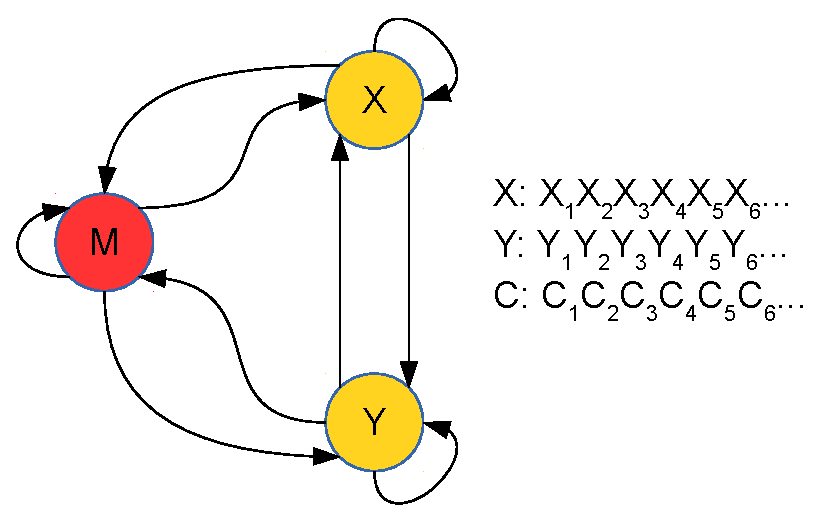
\includegraphics[width=.5\textwidth]{images/model_clf_paska}
    \caption{Model s klasifikátorovou páskou}
\end{figure}


Tento model je síce narozdiel od predošlého korektný pravdepodobnostý model, no má však jednu nevýhodu. Že okrem prípadov, keď klasifikátor vráti hodnotu blízku 0 -- teda tvrdí, že dané 2 pozície by nemali byť zarovnané k sebe (resp. daná pozícia by nemala byť zarovnaná k medzere), penalizuje aj prípady kedy klasifikátor vracia hodnoty blízke 1. Je to z dôvodu, že HMM sa trénuje pomocou frekvenčnej analýzy a pozícií, kde sa vyskytujú hodnoty blízke 1 je menej ako pozícií s hodnotami okolo 0.7.

V tomto modeli sme trénovali aj tranzície aj emisie. Klasifikátorovú pásku sme generovali pomocou oboch klasifikátorov, pričom v Match stave sme použili Match klasifikátor a v Insert stavoch InDel klasifikátor.
Výstupy z klasifikátora sme rozdelili do 10 košov rovnomerne na intervale <0, 1>
